%%%%%%%%%%%%%%%%%%%%%%%%%%%%%%%%%%%%%%%%%
% Masters/Doctoral Thesis
% LaTeX Template
% Version 2.5 (27/8/17)
%
% This template was downloaded from:
% http://www.LaTeXTemplates.com
%
% Version 2.x major modifications by:
% Vel (vel@latextemplates.com)
%
% This template is based on a template by:
% Steve Gunn (http://users.ecs.soton.ac.uk/srg/softwaretools/document/templates/)
% Sunil Patel (http://www.sunilpatel.co.uk/thesis-template/)
%
% Template license:
% CC BY-NC-SA 3.0 (http://creativecommons.org/licenses/by-nc-sa/3.0/)
%
%%%%%%%%%%%%%%%%%%%%%%%%%%%%%%%%%%%%%%%%%

%----------------------------------------------------------------------------------------
%	PACKAGES AND OTHER DOCUMENT CONFIGURATIONS
%----------------------------------------------------------------------------------------

\documentclass[
11pt, % The default document font size, options: 10pt, 11pt, 12pt
%oneside, % Two side (alternating margins) for binding by default, uncomment to switch to one side
english, % ngerman for German
singlespacing, % Single line spacing, alternatives: onehalfspacing or doublespacing
oneside, % twoside
%draft, % Uncomment to enable draft mode (no pictures, no links, overfull hboxes indicated)
%nolistspacing, % If the document is onehalfspacing or doublespacing, uncomment this to set spacing in lists to single
%liststotoc, % Uncomment to add the list of figures/tables/etc to the table of contents
%toctotoc, % Uncomment to add the main table of contents to the table of contents
%parskip, % Uncomment to add space between paragraphs
%nohyperref, % Uncomment to not load the hyperref package
headsepline, % Uncomment to get a line under the header
%chapterinoneline, % Uncomment to place the chapter title next to the number on one line
%consistentlayout, % Uncomment to change the layout of the declaration, abstract and acknowledgements pages to match the default layout
]{MastersDoctoralThesis} % The class file specifying the document structure

\usepackage[utf8]{inputenc} % Required for inputting international characters
\usepackage[T1]{fontenc} % Output font encoding for international characters
\usepackage{cite}

\usepackage{mathpazo} % Use the Palatino font by default

% \usepackage[backend=bibtex,style=authoryear,natbib=true]{biblatex} % Use the bibtex backend with the authoryear citation style (which resembles APA)

% \addbibresource{mscthesis.bib} % The filename of the bibliography

\usepackage[autostyle=true]{csquotes} % Required to generate language-dependent quotes in the bibliography

%----------------------------------------------------------------------------------------
%	MARGIN SETTINGS
%----------------------------------------------------------------------------------------

\geometry{
	paper=a4paper, % Change to letterpaper for US letter
	inner=2.5cm, % Inner margin
	outer=3.8cm, % Outer margin
	bindingoffset=.5cm, % Binding offset
	top=1.5cm, % Top margin
	bottom=1.5cm, % Bottom margin
	%showframe, % Uncomment to show how the type block is set on the page
}

%----------------------------------------------------------------------------------------
%	THESIS INFORMATION
%----------------------------------------------------------------------------------------

\thesistitle{Identifying signatures of human epigenetic modifications among tissues} % Your thesis title, this is used in the title and abstract, print it elsewhere with \ttitle
\supervisor{Thomas \textsc{Bataillon}} % Your supervisor's name, this is used in the title page, print it elsewhere with \supname
\examiner{} % Your examiner's name, this is not currently used anywhere in the template, print it elsewhere with \examname
\degree{Master's in Bioinformatics} % Your degree name, this is used in the title page and abstract, print it elsewhere with \degreename
\author{Alejandro \textsc{Roca Arroyo}} % Your name, this is used in the title page and abstract, print it elsewhere with \authorname
\addresses{} % Your address, this is not currently used anywhere in the template, print it elsewhere with \addressname

% \subject{Biological Sciences} % Your subject area, this is not currently used anywhere in the template, print it elsewhere with \subjectname
\keywords{} % Keywords for your thesis, this is not currently used anywhere in the template, print it elsewhere with \keywordnames
\university{\href{https://www.au.dk/}{Aarhus University}} % Your university's name and URL, this is used in the title page and abstract, print it elsewhere with \univname
\department{\href{http://birc.au.dk/}{Bioinformatics Research Centre}} % Your department's name and URL, this is used in the title page and abstract, print it elsewhere with \deptname
\group{\href{http://birc.au.dk/}{BiRC}} % Your research group's name and URL, this is used in the title page, print it elsewhere with \groupname
\faculty{\href{http://scitech.au.dk}{Faculty of Science and Technology}} % Your faculty's name and URL, this is used in the title page and abstract, print it elsewhere with \facname

\AtBeginDocument{
\hypersetup{pdftitle=\ttitle} % Set the PDF's title to your title
\hypersetup{pdfauthor=\authorname} % Set the PDF's author to your name
\hypersetup{pdfkeywords=\keywordnames} % Set the PDF's keywords to your keywords
}

\begin{document}

\frontmatter % Use roman page numbering style (i, ii, iii, iv...) for the pre-content pages

\pagestyle{plain} % Default to the plain heading style until the thesis style is called for the body content

%----------------------------------------------------------------------------------------
%	TITLE PAGE
%----------------------------------------------------------------------------------------

\begin{titlepage}
\begin{center}

\vspace*{.06\textheight}
{\scshape\LARGE \univname\par}\vspace{1.5cm} % University name
\textsc{\Large Master Thesis}\\[0.5cm] % Thesis type

\hrulefill\ % Horizontal line
\vspace{0.4cm}

{\huge \bfseries \ttitle\par}\vspace{0.4cm} % Thesis title

\hrulefill\
\vspace{1.5cm} % Horizontal line

\begin{minipage}[t]{0.4\textwidth}
\begin{flushleft} \large
\emph{Author:}\\
\href{mailto:alekss.ro@gmail.com}{\authorname} % Author name - remove the \href bracket to remove the link
\end{flushleft}
\end{minipage}
\begin{minipage}[t]{0.4\textwidth}
\begin{flushright} \large
\emph{Supervisor:} \\
\href{mailto:tbata@birc.au.dk}{\supname} % Supervisor name - remove the \href bracket to remove the link
\end{flushright}
\end{minipage}\\[3cm]

\vfill

\large \textit{A thesis submitted in fulfillment of the requirements\\ for the degree of \degreename}\\[0.3cm] % University requirement text
\textit{in the}\\[0.4cm]
\deptname\
\groupname\
\vspace{2cm} % Research group name and department name

\vfill

{\large \today}\\[4cm] % Date
%\includegraphics{Logo} % University/department logo - uncomment to place it

\vfill
\end{center}
\end{titlepage}

%----------------------------------------------------------------------------------------
%	DECLARATION PAGE
%----------------------------------------------------------------------------------------

% \begin{declaration}
% \addchaptertocentry{\authorshipname} % Add the declaration to the table of contents
% \noindent I, \authorname, declare that this thesis titled, \enquote{\ttitle} and the work presented in it are my own. I confirm that:
%
% \begin{itemize}
% \item This work was done wholly or mainly while in candidature for a research degree at this University.
% \item Where any part of this thesis has previously been submitted for a degree or any other qualification at this University or any other institution, this has been clearly stated.
% \item Where I have consulted the published work of others, this is always clearly attributed.
% \item Where I have quoted from the work of others, the source is always given. With the exception of such quotations, this thesis is entirely my own work.
% \item I have acknowledged all main sources of help.
% \item Where the thesis is based on work done by myself jointly with others, I have made clear exactly what was done by others and what I have contributed myself.\\
% \end{itemize}
%
% \noindent Signed:\\
% \rule[0.5em]{25em}{0.5pt} % This prints a line for the signature
%
% \noindent Date:\\
% \rule[0.5em]{25em}{0.5pt} % This prints a line to write the date
% \end{declaration}
%
% \cleardoublepage

%----------------------------------------------------------------------------------------
%	QUOTATION PAGE
%----------------------------------------------------------------------------------------

% \vspace*{0.2\textheight}
%
% \noindent\enquote{\itshape Thanks to my solid academic training, today I can write hundreds of words on virtually any topic without possessing a shred of information, which is how I got a good job in journalism.}\bigbreak
%
% \hfill Dave Barry

%----------------------------------------------------------------------------------------
%	ABSTRACT PAGE
%----------------------------------------------------------------------------------------

\begin{abstract}
\addchaptertocentry{\abstractname} % Add the abstract to the table of contents

\

The number of different epigenetic landscapes for a genome may be inestimable, but we can find correlations between specific epigenetic modifications which are typically associated in concrete functions and development states. In such a way, we reduce the dimensionality of the problem making it easier to draw conclusions from the analysis of the epigenetic modifications, as well as being able to use the smaller set of correlated modifications (or signatures) as input for predictive modelling or supervised machine learning analysis.

\

In order to achieve this, we need to map epigenetic modification reads (from Bisulfite-seq; DNA methylations, or ChIP-seq; histone modifications) into the human genome, specifically into genes and flanking/regulatory regions, which are the ones of interest. In this way we would obtain the counts of each epigenetic modification for different tissues. Non-negative Matrix Factorization (NMF) reveals as an ideal method for the task of finding combinatorial patterns of epigenetic modifications. We can then study the state of each epigenetic modification type in the defined loci of the tissue. From this information we would obtain the different epigenetic signatures which we will use for association and simulation analysis.
\end{abstract}

%----------------------------------------------------------------------------------------
%	ACKNOWLEDGEMENTS
%----------------------------------------------------------------------------------------

% \begin{acknowledgements}
% \addchaptertocentry{\acknowledgementname} % Add the acknowledgements to the table of contents
% The acknowledgments and the people to thank go here, don't forget to include your project advisor\ldots
% \end{acknowledgements}

%----------------------------------------------------------------------------------------
%	LIST OF CONTENTS/FIGURES/TABLES PAGES
%----------------------------------------------------------------------------------------

\tableofcontents % Prints the main table of contents

\listoffigures % Prints the list of figures

\listoftables % Prints the list of tables

%----------------------------------------------------------------------------------------
%	ABBREVIATIONS
%----------------------------------------------------------------------------------------

\begin{abbreviations}{ll} % Include a list of abbreviations (a table of two columns)

\textbf{LAH} & \textbf{L}ist \textbf{A}bbreviations \textbf{H}ere\\
\textbf{WSF} & \textbf{W}hat (it) \textbf{S}tands \textbf{F}or\\

\end{abbreviations}

%----------------------------------------------------------------------------------------
%	PHYSICAL CONSTANTS/OTHER DEFINITIONS
%----------------------------------------------------------------------------------------

% \begin{constants}{lr@{${}={}$}l} % The list of physical constants is a three column table
%
% % The \SI{}{} command is provided by the siunitx package, see its documentation for instructions on how to use it
%
% Speed of Light & $c_{0}$ & \SI{2.99792458e8}{\meter\per\second} (exact)\\
% %Constant Name & $Symbol$ & $Constant Value$ with units\\
%
% \end{constants}

%----------------------------------------------------------------------------------------
%	SYMBOLS
%----------------------------------------------------------------------------------------

% \begin{symbols}{lll} % Include a list of Symbols (a three column table)
%
% $a$ & distance & \si{\meter} \\
% $P$ & power & \si{\watt} (\si{\joule\per\second}) \\
% %Symbol & Name & Unit \\
%
% \addlinespace % Gap to separate the Roman symbols from the Greek
%
% $\omega$ & angular frequency & \si{\radian} \\
%
% \end{symbols}

%----------------------------------------------------------------------------------------
%	DEDICATION
%----------------------------------------------------------------------------------------

% \dedicatory{For/Dedicated to/To my\ldots}

%----------------------------------------------------------------------------------------
%	THESIS CONTENT - CHAPTERS
%----------------------------------------------------------------------------------------

\mainmatter{} % Begin numeric (1,2,3...) page numbering

\pagestyle{thesis} % Return the page headers back to the "thesis" style

% Include the chapters of the thesis as separate files from the Chapters folder
% Uncomment the lines as you write the chapters

% Chapter Template

\chapter{Introduction}\label{Intro}   % Change X to a consecutive number; for referencing this chapter elsewhere, use \ref{Intro}

%----------------------------------------------------------------------------------------
%	SECTION 1
%----------------------------------------------------------------------------------------

\section{Epigenetics}

The genetic material is known to be modified during the life of an organism, possibly causing modifications in gene behavior. Far is known about mutations being a mayor player in genetic variation and the profiling of these variations has proved to be highly useful when studying diseases and evolutionary theory \cite{Wray2007}. In eukaryotes, there are in addition mechanisms in which the DNA can be modified without altering the molecular sequence, so called epigenetic mechanisms. As Conrad Waddington, who coined the term ``epigenetics'', defined: ``it is the branch of biology which studies the causal interactions between genes and their products, which bring the phenotype into being'' \cite{Waddington1942}. Such definition led to categorizing as epigenetics all biological phenomena which correlated the genetic material with the genetic products and were not explained entirely by the classic genetic studies. Further studies have revealed that epigenetic mechanisms can be modulated in response to external stimuli \cite{Liu2004,Backdahl2009}, entailing an overlay between DNA  and environment for the cells and organisms. Moreover, the epigenetic mechanisms behavior can vary for different stages of cell development \cite{Kiefer2007}, environmental changes \cite{Sutherland2003} or disease \cite{Jessberger2007}. In the same way genetic variability can be profiled, it is possible to decipher shared patterns for the epigenetic modifications in different scenarios and types of tissue.

\medskip

Due to the latest growth on research efforts and resources about the topic, we were able to characterized the inheritance of gene expression patterns not explained by the encoded information in the DNA sequence but through epigenetic modifications. High-throughput technologies such as Chromatin Inmunoprecipitation next-generation sequencing (ChIP-seq) or Whole-Genome Bisulfite sequencing (WGBS), allowed us to obtain an incredibly vast amount of information on epigenetic marks throughout the genome. It was then possible to determine the epigenome profile consisting of multiple chromatin states that activate or repress the gene expression in a local and cell-specific manner. This ``epigenomic profiling'' helped the understanding of cell differentiation, where even though the vast majority of cells in a multicellular organism share an identical genotype, the development of the various tissues generates stable but diverse profiles of gene expression, giving rise to the multiple cell types and differentiated cellular functions. In light of this, more specifically epigenetics may be defined as “the study of any potentially stable and, ideally, heritable change in gene expression or cellular phenotype that occurs without changes in Watson-Crick base-pairing of DNA” \cite{Goldberg2007}.

\medskip

The work on nucleic acids, chromatin and histone proteins led to the understanding of the DNA arrangement, as being wrapped around the histone proteins, and furthermore to the cytological distinction between euchromatin and heterochromatin \cite{Elgin1996}. It has been proved that post-translational modifications of the histones, such as methylation, acetylation or phosphorylation, can reshape the chromatin structural and functional properties instating the concept of turning ``on'' and ``off'' regions of the genetic material. A challenging yet feasible task is to characterize those configurations responsible for the repression, activation or modulation of the gene expression via epigenetic modifications, both in different tissues and also when affected by diseases as in the case of the cancer cells used in this study. For further understanding, it is essential to know about the diverse ways epigenetic mechanisms work and elucidate the correlation among them and to biological processes.

%-----------------------------------
%	SUBSECTION 1
%-----------------------------------
\subsection{Epigenetic modification types}

\subsubsection{Histone Modifications}

Chromatin is conformed by the DNA molecule and a range of binding proteins into which histones are included. The DNA molecule winds around an octamer of histones, formed by dimers of four core histones: H2A, H2B, H3 and H4. Histone N-terminal tails, specially long in Histone 3 (H3), are subject of chemical modifications, such as methylation or acetylation, modulating their spatial configuration and with it, the arrangement of the chromatin. First works on the subject, in particular on histone acetylation \cite{Schatz1964}, implied a close linkage between the histone modification state and the local gene activity. This assumption was afterwards supported by experiments on histone-tail mutations in \textit{Saccharomyces cerevisiae} \cite{Kayne1988}, hypoacetylation of the inactive X chromosome in female mammals \cite{Jeppesen1993}, as well as hyperacetylation of the twofold upregulated X chromosome in \textit{D. melanogaster} males \cite{Bone1994}. These major findings led to the compelling argument that histone modifications, along with DNA methylation, contribute to distinguish between euchromatin state and heterochromatin. Accordingly, depending on the particular histone modification profile, the chromatin can be arranged as euchromatin, which implies gene expression, or as heterochromatin, meaning the repression of the gene activity.

\medskip

Chromatin state at promoters is largely invariant across diverse cell types, whereas enhancers are marked with highly cell-type-specific histone modification patterns \cite{Heintzman2009}. As in methylation patterns, an aberrant histone modification pattern is associated with the development of cancer \cite{Barneda-Zahonero2012}. Histone deacetylases (HDACs) are implicated expecting both positive and negative effects on oncogenic and oncosuppressive mechanisms. Again, the importance of the histone modification patterns for the gene expression and the diseases associated with an aberrant histone modification profile, call our attention on the topic.

\subsubsection{DNA methylation}

DNA methylation is perhaps the best characterized chemical modification of chromatin and were detected as early as 1948 \cite{HOTCHKISS1948}. In mammals, nearly all DNA methylation occurs on cytosine residues of CpG dinucleotides. Regions of the genome that have a high density of CpGs are referred to as CpG islands, and DNA methylation of these islands correlates with transcriptional expression \cite{Deaton2011}. De novo or maintenance DNA methyltransferases (DNMTs) play a critical role in gene regulation, especially those associated with transposons and imprinted genes \cite{Goll2005}, by keeping the genomic patterns of cytosine methylation during embryogenesis and gametogenesis. Moreover, the formation of heterochromatin in several organisms is mediated partly by DNA methylation and its binding proteins together with RNA and histone modifications. DNA methylation takes part in many cellular processes including silencing of repetitive and centromeric sequences from fungi to mammals \cite{Partridge2002,Jones2012}; X chromosome inactivation in female mammals \cite{Weber2005}; and mammalian imprinting \cite{Bartolomei2011}, all of which can be stably maintained.

\medskip

As the other epigenetic mechanisms, DNA methylation is reversible and therefore DNA methylation patterns vary in time and space during differentiation \cite{Jones1980,Xie2013}. However, abnormal control of the methylation pattern was detected in cancer cells and may result in the generation of random modification patterns which may serve to unleash new genes for transcription \cite{Berdasco2010}. The abnormal methylation pattern can be either hypomehylated, which usually involves repeated DNA sequences, or hypermethylated which involves CpG islands \cite{Weber2005}. In the first case, oncogenes are activated whereas hypermethylation repress the transcription of the promoter regions of tumor suppressor genes, leading to gene silencing.

\subsubsection{RNA-Associated Silencing}

RNA silencing is another method to turn off genes when it is in form of antisense transcripts, noncoding RNAs or RNA interference. Antisense double-stranded RNA complementary to targeted mRNAs was detected as a method of Post-Transcriptional gene silencing (PTGS) for both cellular and viral genes in a sequence-specific manner \cite{Hamilton1999}. This kind of process is known as RNA-mediated interference or RNAi. Moreover, small non-coding RNAs were identified as potencial `templating' molecules for the location-specific epigenetic modifications. Several researches reported the involvement of small nuclear RNAs (snRNAs) in interacting with and presumably directing chromatin-modifying activities \cite{Mochizuki2002,Borges2015}. The snRNAs participate in a nuclear process known as `transcriptional gene silencing' (TGS) guiding the epigenetic machinery not only for heterochromatin assembly and gene silencing \cite{Grewal2003}, but also directing programmed DNA elimination \cite{Bernstein2005}.

\subsubsection{Alternative Splicing}

Alternative splicing is one major mechanism that makes the most of the precursor messenger RNAs (pre-mRNAs) by processing the pre-mRNA into a diverse array of mature mRNAs that encode distinct proteins. This phenomenon explains the high complexity of organisms as humans while they have a relatively small number of protein-coding genes. Alternative splicing of RNA leads to a variety of possible mRNA isoforms and proteins, which can have different, and often opposing, functions. Sequences called exons are regions of the pre-mRNA that are included in the mature mRNA, such as the protein-coding sequences and regulatory untranslated regions at either end of the mRNA.\@ Sequences called introns are the portions of the pre-mRNA that are removed during splicing. In alternative splicing, some sequences serve as exons under some conditions and are included in the final mRNA.\@ At other times, however, the alternative splicing process may exclude the same sequence, treating it as an intron and removing it from the mature mRNA.\@

\medskip

A critical finding regarding the prevalence of alternative splicing was that a majority of human genes produce a wide variety of messenger RNAs (mRNA) that in turn encode distinct proteins \cite{Johnson2003}. Scientists estimate that 15–60 percent of human genetic diseases involve splicing mutations, either through direct mutation of the splice-site signals or through disruption of other components of the splicing pathway \cite{Wang2007}. Therefore, understanding how the splicing machinery distinguish between exons, which are part of the mature mRNA, and introns, which are removed from the pre-mRNA, is of critical importance. Alternative splicing adds an extra layer of complexity, because regulatory sequences that sometimes designate an exon's inclusion into the mature mRNA dictate the exclusion of that exon under other conditions.

%-----------------------------------
%	SUBSECTION 2
%-----------------------------------

\subsection{Epigenomic modeling}

% Explain previous attempts on modeling the epigenetic profiles and where did they focus

% Origin of epigenetic modeling

Mentioned growth on epigenetics data availability, favored by the arise of NGS sequencing techniques, granted the possibility to create extensive descriptions on the different epigenetic marks for various samples. Moreover, the findings on the function of epigenetic modifications to modulate the chromatin arrangement provided a glimpse of the likeliness to characterize the relationships between chromatin states and gene expression profiles. Thanks to the contribution made to the two major public databases, the ENCODE (The ENCyclopedia of Dna Elements) \cite{Feingold2004} and the NIH Roadmap Epigenomics \cite{Bernstein2010}, this characterization becomes more accessible. Modeling the epigenetic modifications requires the development of computational tools which use the multiple types of data, such as DNA methylation, histone modification or Transcription Factors (TFs), in order to establish a correlation between the epigenomic assays and the biological activity. The main objectives of finding the specified models are both learn more about the biological association of epigenetic modifications and which predictions can be achieved from the models. The nature of the algorithms used to model epigenomics have been diverse but most of the proposed methods fall under unsupervised learning techniques of classification, which seek to devise patterns of chromatin modifications from the datasets alone, relying for it on multiple statistical techniques.

\medskip

A first proper mathematical attempt to model histone modification dynamics was made in \cite{Dodd2007}, where they characterized the bistable gene expression resulting from the alternative states of the chromosomal regions. They applied a simple stochastic model in which they divided the DNA into \~1.2 kb, corresponding to around 60 nucleosomes, and they consider either modified or unmodified nucleosomes from which they try to infer the state conversion of a region. Further contributions delved into the pattern-finding idea using more complete models such in ChromaSig \cite{Hon2008}. Nine different types of epigenetic marks were taken into account in order to find strong signals of correlation between the epigenetic signatures profile and the promoter and enhancer activity state. Nevertheless, the analysis worked on a pre-defined set of loci with high grade of epigenetic modifications from the ENCODE project pilot, representing only the 1\% of the human genome \cite{ENCODEProjectConsortium2007}. The essence of the method requires to calculate the likelihood for each loci towards being classified in a motif by using an euclidean distance measure. On account of the computational limitations, these methods could not be applied to study whole-genome marks and on multiple genomic assays.

\medskip

More recent tools are able to directly specify the combination of epigenetic modifications or `chromatin states' in a genome-wide fashion, making use of integrative models based on Hidden Markov Models (HMM) like in ChromHMM \cite{Ernst2010,Ernst2017} and EpicSeg \cite{Mammana2015}, or dynamic Bayesian networks like in Segway \cite{Hoffman2012}. ChromHMM software learns and characterizes the chromatin states from multiple ChIP-seq datasets by creating tracks of presence/absence vectors for the epigenetic mark in a k-binned genome. In such a way, genome-wide annotation is efficient but it misses the quantitative hand of the epigenetic mark reads, using only binary data. EpicSeg uses a similar angle in the analysis, however there is no need to pre-process the data as it uses raw read counts like observations in the analysis, which allows to define a valid discrete multivariate probability distribution and then solve the lost of quantitative data. For its part, Segway refuses the idea of genome segmentation and addresses the most probable sequence of chromatin states by means of a Dynamic Bayerian Network (DBN) at a 1-bp resolution. This approach can elucidate some limitations from previous methods such as missing data handling or finding the correct constrains for segments length.

\medskip

Yet, there are practical limitations essentially about the precondition to define the number of chromatin states beforehand, since this choice is arbitrary from the model and answers to biological interpretability of the results. Moreover, the algorithms mentioned above are computationally intensive and challenging to use without a sufficiently computational power. A relatively new statistical method called Non-Negative Matrix Factorization (NMF) \cite{Lee1999} has been applied to the problem in question of finding chromatin states from the reads of epigenetic modification marks \cite{Cieslik2014,Gandolfi2017}. NMF undertake the dimensionality problem on the genome-wide analysis of epigenetic tracks by approximating the dataset values through a reduced number of meaningful components \cite{Devarajan2008}. The method makes it possible to integrate multiple epigenetic marks to the characterization of chromatin combinatory patterns, and also allows to find an optimal number of distinct patterns based on the data. In both studies \cite{Cieslik2014,Gandolfi2017}, they applied NMF to matrices consisting on multiple epigenetic marks as columns and non-overlapping segments of the genome as rows, being the value of the cell equal to the read counts.

\medskip

In the first case, the segments used as rows correspond to multiple regions of TSS-proximal gene bodies since they contain epigenetic traces of transcription initiation and elongation. In the second case, they use bins of 200-bp, similar to the case in ChromHMM, in an attempt to approximate a single nucleosome with each bin. In the present study, aspects from these papers were used, extending the analysis to multiple cancer cell lines.

%----------------------------------------------------------------------------------------
%	SECTION 2
%----------------------------------------------------------------------------------------

\section{Non-negative Matrix Factorization}

Non-negative matrix Factorization reveals as a method to learn parts or components from high-dimensional data. In contrast to other matrix factorization methods such as Principal Component Analysis (PCA) or Vector Quantization (VQ), NMF does not learn holistic but part-based representations. In addition, NMF is constrained to have positive values as only additive combinations are considered \cite{Lee1999}. Basically, NMF consists on an approximation of an \(m \times n\) \(V\) matrix by the matrix multiplication of \(W\) (\(m \times k\)) and \(H\) (\(k \times n\)).

\begin{equation}
    V \approx W \times H
\end{equation}

This shall be accomplished by iteratively updating the rows and columns of \(W\) and \(H\) respectively. The constriction of the data to be positive also circumscribe the use of the method, though it has been applied in astronomy \cite{Ren2017}, language processing \cite{Bertin2010} or image processing \cite{Yang2007} among others. Gene expression, epigenetic modifications or mutation data have also been subject of analysis using NMF, considering the non-negativity of the data.

\medskip

Dealing with high dimensionality data using NMF implies taking certain decisions, starting from the choice of NMF dimensionality (number of \(k\) signatures). An important measure used for this task is the reconstruction error, calculated by comparing the original data value with the result of the multiplication of the factorized matrices \(W\) and \(H\). Some of the studies compare the reconstruction error produced by each defined \(k\) using the real data vs the one produced when taking random data, as it is the case in this analysis \cite{Frigyesi2008}. When examining the Residual Sum of Squares (RSS) as a function of \(k\), the RSS decreases with increasing \(k\) within the original dataset, however, this can be less the case for the random dataset. Ideally, for a given interval of \(k\) values, there ought to be an optimal \(k\) for which the slopes of the real and random data intersect. That is to say, we intend to find the highest \(k\), reducing the reconstruction error and improving the accuracy of the model, before being within the noise. Other studies use the cophenetic correlation coefficient, where the similarity between results from several runs is compared for each \(k\). In other words, the stability of the classification is studied choosing the highest \(k\) before the robustness of the results drops \cite{Brunet2004}.

\subsection{NMF algorithms}\label{NMFalgs}

Within NMF method we find several ways of solving the factorization problem of form \(V \approx W H\). Again, the non-negativity constrain makes previous factorization approaches not applicable and then new algorithms needed to be developed. First approaches \cite{Lee2001} were based on minimizing either the euclidean distance between \(V\) and \(WH\) such that

\begin{equation}
    \vert \vert V - WH \vert \vert ^2 = \sum_{ij} (V_{ij} - (WH)_{ij})^2
\end{equation}

or minimizing the divergence between \(V\) and \(WH\),

\begin{equation}
    D(V \vert \vert WH) = \sum_{ij}\left(V_{ij} \log \frac{V_{ij}}{(WH)_{ij}} - V_{ij} + (WH)_{ij} \right)
\end{equation}

as in both cases, the measure is lower bounded by zero and minimizes when \(V = WH\). Once the cost function for the minimization was defined, multiplicative rules were proposed as the procedure to update \(W\) and \(H\). A compelling property of the approximation is that (1.1) can be reformulated in a column or row-wise manner:

\begin{itemize}
    \item Update columns in \(H\): \(v \approx Wh\) when \(v\) represents a column in \(V\), \[v = (V_{1n}, \ldots , V_{Mn}) \in \mathbb{R}^M\], and \(h\) a column in \(H\), \[h = (H_{1n}, \ldots , H_{Kn}) \in \mathbb{R}^K\]
    \item Update rows in \(W\): \(v \approx wH\) when \(v\) represents a row in \(V\), \[v = (V_{1m}, \ldots , V_{Nm}) \in \mathbb{R}^N\] and \(w\) a row in \(W\) \[w = (W_{1m}, \ldots , W_{Km}) \in \mathbb{R}^K\]
\end{itemize}

Therefore, it is possible to iteratively update rows in \(W\) and then columns in \(H\). The multiplicative updates for \(H\) and \(W\) in the euclidean distance minimization were described with the next form \cite{Lee2001}:

\begin{equation}
    H_{kj} \leftarrow H_{kj} \frac{(W^T V)_{kj}}{(W^{T}WH)_{kj}	}
\end{equation}

\begin{equation}
    W_{ik} \leftarrow W_{ik} \frac{(V H^T)_{ik}}{(WHH^T)_{ik}}
\end{equation}

and the multiplicative updates for the divergence, based on Kullback-Leibler divergence, and subsequently applied to retrieve meaningful patterns from cancer gene expression data \cite{Brunet2004}, were described as follows:

\begin{equation}
    H_{kj} \leftarrow H_{kj} \frac{\sum_l \frac{W_{lk} V_{ij}}{(WH)_{ij}}}{\sum_l W_{lk}}
\end{equation}

\begin{equation}
    W_{ik} \leftarrow W_{ik} \frac{\sum_l \left[ \frac{H_{kl} V_{ij}}{(WH)_{il}} \right]}{\sum_l W_{kl}}
\end{equation}

Proofs of these theorems and convergence rules are further explained in \cite{Lee2001}. After these principle algorithms, some approaches were developed based on them in order to get sparser results \cite{Pascual-Montano2006} or include an intercept into the NMF fit \cite{Badea2008}.

\subsection{NMF and gene expression}

NMF was promptly introduced in bioinformatics as a method of dimensionality reduction of large-scale gene expression data \cite{Kim2003}. Here, functional relationships are yield from the analysis of 300 genome-wide expression measurements of yeast and compared with previous expertise. The 5346 genes analyzed in 300 samples were summarized in 50 patterns from which 12 were annotated with MIPS \cite{Mewes2002} functional categories, based on the frequency which genes from each category appeared in each of the signatures or patterns. In a similar way, NMF has also been applied to categorize tumor subtypes using 4651 human genes in 108 cases \cite{Frigyesi2008}, showing that NMF signatures may correspond specific disease gene expression patterns.

\subsection{NMF and mutations}

Besides finding shared patterns between diseases and gene expression, it has been shown that it is possible to characterize specific mutations produced in varied types of cancer \cite{Ramakrishna2012}. A catalogue of complete genomes for 21 primary breast cancer samples was sequenced and compared to the normal DNA of those same individuals. From these, 183,916 somatically acquired mutations were called and classified into 96 possible trinucleotide variations, composing the \(V\) matrix of \(183916 \times 21\) cells. NMF was then applied on this dataset and from the results they identified contribution of each of the mutational signatures in each of the patients, which yield similar arrangement for similar cancer types.

\medskip

Although the number of identified signatures was five, further on this number got reduced to only four signatures \cite{Alexandrov2013}. In such a way, mutational processes operative in cancer genomes were modeled with great accuracy by a combination of this four mutational signatures. This allowed to make predictions based on the signatures and the data, as well as understand more deeply the biological processes involved on the different types of cancer.

\subsection{NMF and epigenetics}

The epigenetic modeling techniques explained before have shown the possibility to find genome-wide chromatin states based on the partition of the DNA. Nevertheless, they make the assumption that a small set of these chromatin states would be sufficient to describe the genomic expression, whereas several hundreds chromatin states have been estimated even with a small set of epigenetic marks used \cite{Ucar2011}. In addition, chromatin modifications tend to be highly correlated, hampering the task of assessing the importance of the chromatin marks and relating them to the biological mechanisms. NMF can be used in order to overcome these downsides by identifying combinatorial patterns of chromatin states.

\medskip

This application was initially presented as a way to get combinatorial patterns of epigenetic marks from integrated epigenetic data sets \cite{Cieslik2014}. They characterized a small amount of combinatorial patterns, which could be displayed and interpreted, were statistically capable of regression and classification tasks. Each row of the \(V\) matrix represents 2 kbp of regions flanking Transcription Start Sites (TSS) and columns represent the epigenetic marks used. In a case study for regression of \textit{Pol2} binding, ten epigenetic marks were used to identify seven quantitative epigenetic patterns. Using the 7 chromatin patterns in a regression model yield a performance of \( r^2 = 0.85 \), matching the one obtained by using 10 epigenetic marks but solving multicollinearity problems.

\medskip

Later on, functional classification of the epigenome was performed by adding more epigenetic marks and in this case, segmenting the DNA into 200 bp regions as an attempt to resemble one nucleosome with each 200-bp bin \cite{Gandolfi2017}. NMF was here applied to 13 different epigenetic marks over 833,738 significant bins in human embryonic stem cells, finding 7 epigenetic signals or chromatin profiles. These seven epigenetic signals were then labeled based on the related biological process and then used for a wide range of tasks: study the genomic distribution of the signatures, investigate their recovery power on genomic features, association with the gene expression \ldots

\medskip

Over the present analysis, aspects of these previous analysis have been reproduced, adopting the processing of the data scheme \cite{Gandolfi2017}, segmenting the genome into 200-bp bins and extending the analysis to three cancer cell types for which eleven common epigenetic marks were available. Results show that there are similar chromatin signatures found for these tissues, suggesting a possible generalization of the chromatin profiles in normal and cancer cells.

% Chapter Template

\chapter{Methods}\label{Methods} % for referencing this chapter elsewhere, use \ref{Methods}

%----------------------------------------------------------------------------------------
%	SECTION 1
%----------------------------------------------------------------------------------------

\section{NMF}

Non-Negative Matrix Factorization is the statistical framework in which this analysis is based on. Given a non-negative matrix \(V\), NMF is an unsupervised learning method which tries to find non-negative matrix factors \(W\) and \(H\) such that

\begin{equation}
     V \approx W \times H.
\end{equation}

The epigenetic data used, described in a later section, fulfills the precondition of non-negativity of the data. The \(V\) matrix used in the analysis is composed by 200-bp bins as rows and the epigenetic marks as columns. We are investigating the possibility of finding \(k\) signatures which will summarize combinatorial patterns of the data to the epigenetic marks by means of the \(H\) matrix and to the genome-wide bins by means of the \(W\) matrix.

\medskip

In order to perform the analysis, the \(V\) matrix was loaded into R environment and concretely the Rpackage \textit{NMF} was used \cite{Gaujoux2010}. The package used was select for consistency with previous similar studies \cite{Gandolfi2017} and seeing that attempts to implement the algorithm resulted in more time-consuming alternatives. Rpackage \textit{NMF} offers a framework with several NMF algorithms, including the ones explained in a previous section, from which \texttt{brunet} option was chosen. This algorithm is based on Kullback-Leibler divergence and matches the one described in \cite{Lee2001} and used in \cite{Brunet2004}, enhanced to avoid numerical overflow.

%-----------------------------------
%	SUBSECTION 1
%-----------------------------------
\subsection{Algorithm}

Passed on a non-negative matrix \(V\) of \(m \times n\) size and a chosen number of \(k\) signatures, \texttt{brunet} implementation will find the approximation \(V \approx WH\).

\begin{enumerate}
    \item First, both \(W\) and \(H\) matrices are randomly initialized.
    \item Then, every row in \(W\) is updated according to the correspondent multiplicative update rules mentioned in (1.7).
    \item Every column in \(H\) is updated according to (1.6).
    \item Repeat steps 2 and 3 until the default convergence criteria is reached.
\end{enumerate}

The stopping or convergence criteria for the NMF algorithm can be based on a fixed number of iterations or the invariability of the target values \[( \vert \vert WH \vert \vert  )_t = ( \vert \vert WH \vert \vert  )_{t+1}.\] Since no fixed number of iterations was assumed, the stopping criteria for the analysis was the invariability of the \(WH\) matrix multiplication, which means there were different number of iterations when NMF was applied to the alternative tissues, varying between 350-600 iterations. The implementation in \textit{NMF} package includes parallel computations to speed up the process.

%-----------------------------------
%	SUBSECTION 2
%-----------------------------------

\subsection{Choosing number of signatures}

Explain different ways to choose N, the way used, the N used and why.

%----------------------------------------------------------------------------------------
%	SECTION 2
%----------------------------------------------------------------------------------------

\section{Data}

The data used in this study is obtained entirely from the ENCODE project database \cite{Feingold2004}, where multiple epigenetic marks and reference epigenomes are available. Data sets from 11 types of epigenetic marks were collected, including histone modifications (H3K4me3, H3K4me1, H3K27ac, H3K36me3, H3K9me3, H3K27me3 and H3K9ac), chromatin remodeling proteins (EP300 and H2A.Z) and transcription regulation factors (CTCF, POLR2A). Replicate samples for each of the 11 epigenetic marks were used in the three cell lines of study, which includes a human liver cancer cell line (HepG2) \cite{Aden1979}, myelogenous leukemia cell line (K562) \cite{Andersson1979} and cells derived from HeLa cancerous cervical tumor line (HeLa-S3) \cite{Douglas1973,Chen2008}.

\medskip

In order to standardize the input and facilitate the data sets processing, the information for all the samples was arranged in a tab separated file with the following fields as columns:

\begin{enumerate}
    \item \textbf{Cell line type}. Either HepG2, K562 or Hela-S3.
    \item \textbf{Epigenetic modification category}. Where does the modification apply. Either histone modification (`histonemod'), chromatin modulation (`openchromatin') or transcription factor (`TFBS').
    \item \textbf{Epigenetic modification name}. The label of the mark which the sample corresponds to, as mentioned above.
    \item \textbf{Accession ID}. The accession name for the sample in the database.
    \item \textbf{File name}.
    \item \textbf{Processing status}. Either `raw' or `process'. Raw samples need to be pre-processed.
    \item \textbf{Replicate number}. Integer enumerating the various replicates for a particular epigenetic mark.
    \item \textbf{Database name}. In the present case, `ENCODE'.
    \item \textbf{Download link}. Used to download the sample reads file.
\end{enumerate}

As a matter of convenience, `\path{downloadData.sh} \path{[DataInfo.tsv]}' or `\path{epigeNMF.sh} \path{-d}  \path{[DataInfo.tsv]}' can be used to automatically download the data sets into the appropriate directory tree: \path{CELL_LINE/SIGNAL_TRACK/SAMPLE_ID}.

%----------------------------------------------------------------------------------------
%	SECTION 4
%----------------------------------------------------------------------------------------

\section{Pipeline}

Explain the command line tool, the pipeline followed for the analysis and explain functioning of each script

You should follow the next pipeline for the analysis:

\begin{enumerate}
    \item Download the data (option \path{-d} or \path{--download})
    \item Prepare BED alignment files (option \path{-p} or \path{--process})
    \item Create V matrix of counts for marks (cols) by bins (rows) (option \path{-c} or \path{--counts})
    \item Filter V matrix bins to remove noise (option \path{-f} or \path{--filter})
    \item Choose the optimal `n' number of signatures for NMF (option \path{-k} or \path{--chooseN})
    \item NMF analysis (option \path{-n} or \path{--nmf})
\end{enumerate}

\section{Performance}

Perform analysis with percentage of the data and get performance (time) plots

% Chapter Template

\chapter{Results}\label{Results} % for referencing this chapter elsewhere, use \ref{Results}

%----------------------------------------------------------------------------------------
%	SECTION 1
%----------------------------------------------------------------------------------------

\section{NMF Signatures}

The NMF produces two factorized matrices, \(H\) and \(W\). Among them, \(H\) matrix is the one that relates the epigenetic marks to the signatures, giving a \(7 \times 11\) array. From this matrix, we can study the combinatorial relations between the epigenetic modifications. One important aspect to bear in mind is that the signatures which yield from the method do not come off in the same order. This is due to the random initialization of the matrices. Therefore, referring to particular signature numbers in the following lines is just used for comparison purposes. A good way to compare the \(H\) matrix outcome is by analyzing the values in it using a heatmap plot. In order to relate the signatures from the different cell tissues, correlation between their values was used.

\begin{figure}[h!]
    \centering
    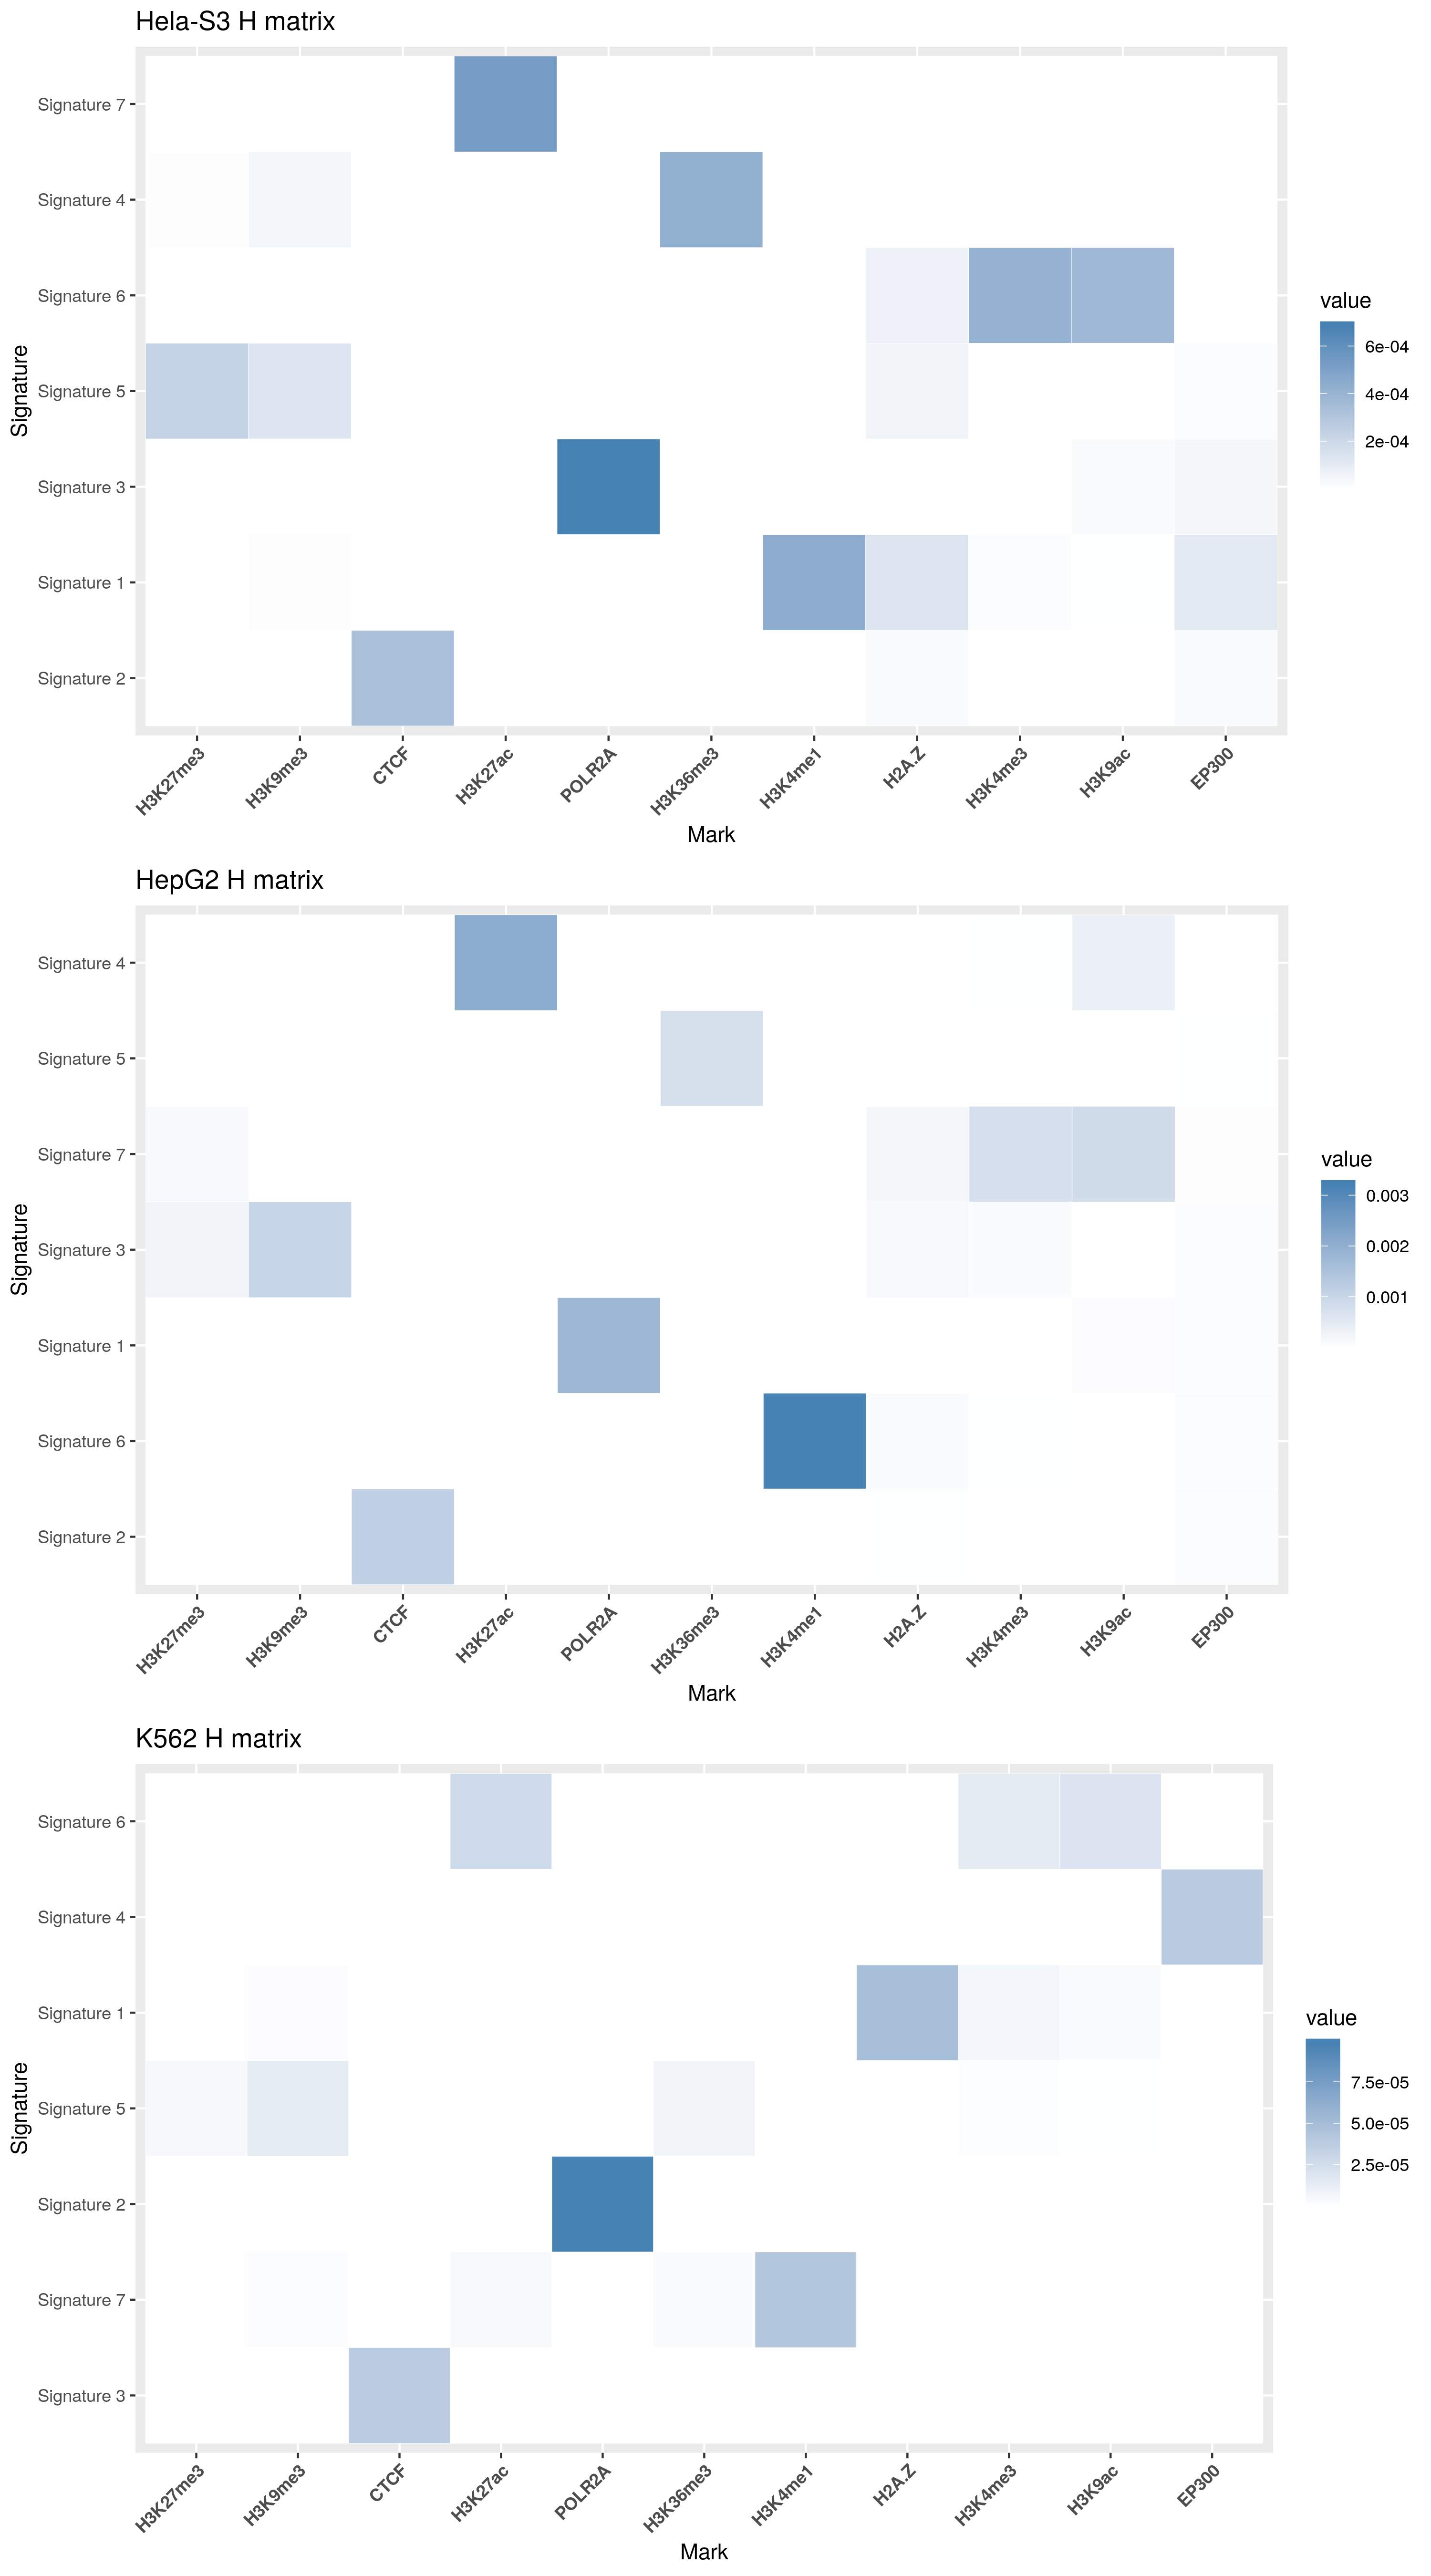
\includegraphics[width=0.8\textwidth]{Figures/NMF/vert_comb.png}
    \caption[Heatmap of the obtained H matrices]{\textbf{Heatmap of the obtained H matrices}. Heatmap of the \(W\) matrix weights obtained from NMF algorithm. From top to botton we see the results for the Hela-S3 cell line, HepG2 cells and K562. The signatures were ordered by correlation, which facilitate the comparison between plots.}
    \label{fig:H_heatmaps}
\end{figure}

Figure~\ref{fig:H_heatmaps} shows the \(H\) matrix results for the three cell lines analyzed. The arrangement of the signatures was decided according in order to correspond to the one shown in \cite{Gandolfi2017}. As we can see, there are numerous coincidences between the heatmaps. Assuming we related the signatures correctly, we can adopt the same `genomic labels' for the signatures in the following order from top to bottom: (1) `Active Promoter', (2) `Repressed Chromatin', (3) `Transcription Initiation', (4) `Repressed Regulatory Regions', (5) `Gene Body Transcription',  (6) `Enhancer Regions' and (7) `Regulatory Elements'.

\begin{enumerate}
    \item The `Active Promoter' signature shows a predominance of H3K27ac modification, associated with a higher activation of the gene expression (acts as an active enhancer mark). HepG2 and K562 show in addition importance of the H3K9ac modification, also correlated with active promoters. H3K4me3 is an activation-related modification which also appears to be important in K562 tissue.
    \item In the `Repressed Chromatin' signature in contrast, the predominant marks in Hela-S3 are H3K36me3 and to a lesser extent H3K9me3. H3K36me3 and H3K9me3 are both known to be implicated in the repression of aberrant trancription \cite{Bartke2010}. It is noticeable how in the cancer cells analyzed in this report, it is more predominant the presence of H3K36me3 than H3K9me3 while it is the other way around for the IMR90 cell line. H3K36me3 is known for serving as a mark for the histone descetylases (HDACs) to act in the DNA. This can be related with the amplified action of the HDACs seen in cancer cells.
    \item `Transcription Initiation' includes the presence of H2A.Z, H3K4me3 and H3K9ac, all of them activators when they are localized close to the promotors.
    \item `Repressed Regulatory Regions' signature includes H3K27me3 as in IMR90 but in the cancer cells it is also important H3K9me3, in any case, both related with heterochromatic regions.
    \item `Gene Body Transcription' includes a dominant presence of DNA-directed RNA polymerase II subunit gene (POLR2A).
    \item In the `Enhancer Regions' signature, H3K4me1 stands out for Hela-S3, HepG2 and K562. H3K4me1 is seen as a ``window of opportunity'' for the enhancer activation by modulating nucleosomal mobility through the H2A.Z-containing nucleosomes. This process provokes the chromatin structure to be more dynamic, enhancing the Transcription Factor accessibility. This is consistent with the co-occurrenceof H2A.Z in this signature.
    \item Last, `Regulatory Elements' signature comprise the Transcriptional repressor CTCF.
\end{enumerate}

\section{Signature distribution along the genome}

\begin{figure}[h!]
    \centering
    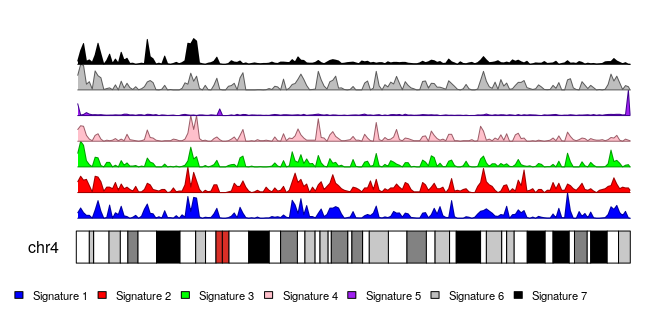
\includegraphics[width=\textwidth]{Figures/cover/chr4.png}
    \caption[Signatures density in chromosome 4]{\textbf{Signatures density in chromosome 4}. Representation of the chromosome 4 and overlay with the density distribution of the signatures. Signature 1 (Active Promoter) is represented in blue, Signature 2 (Repressed Chromatin) in red, Signature 3 (Transcription Initiation) in green, Signature 4 (Repressed Regulatory Regions) in pink, Signature 5 (Gene Body Transcription) in purple, Signature 6 (Enhancer Regions) in grey and Signature 7 (Regulatory Elements) in black}
    \label{fig:chr4}
\end{figure}

The second factorized matrix is the \(W\) matrix, which relates the signatures with the bins and thus with the genome location. In this way, we can associate each of the bins their prevailing signature. Each bin got assigned the signature for which the weight was highest. This been done, the distribution of the signatures along the genome can be represented using a density plot. Figure \ref{fig:W_density} shows an example representation of the signature location along the chromosomes.

\begin{sidewaysfigure}[ht]
    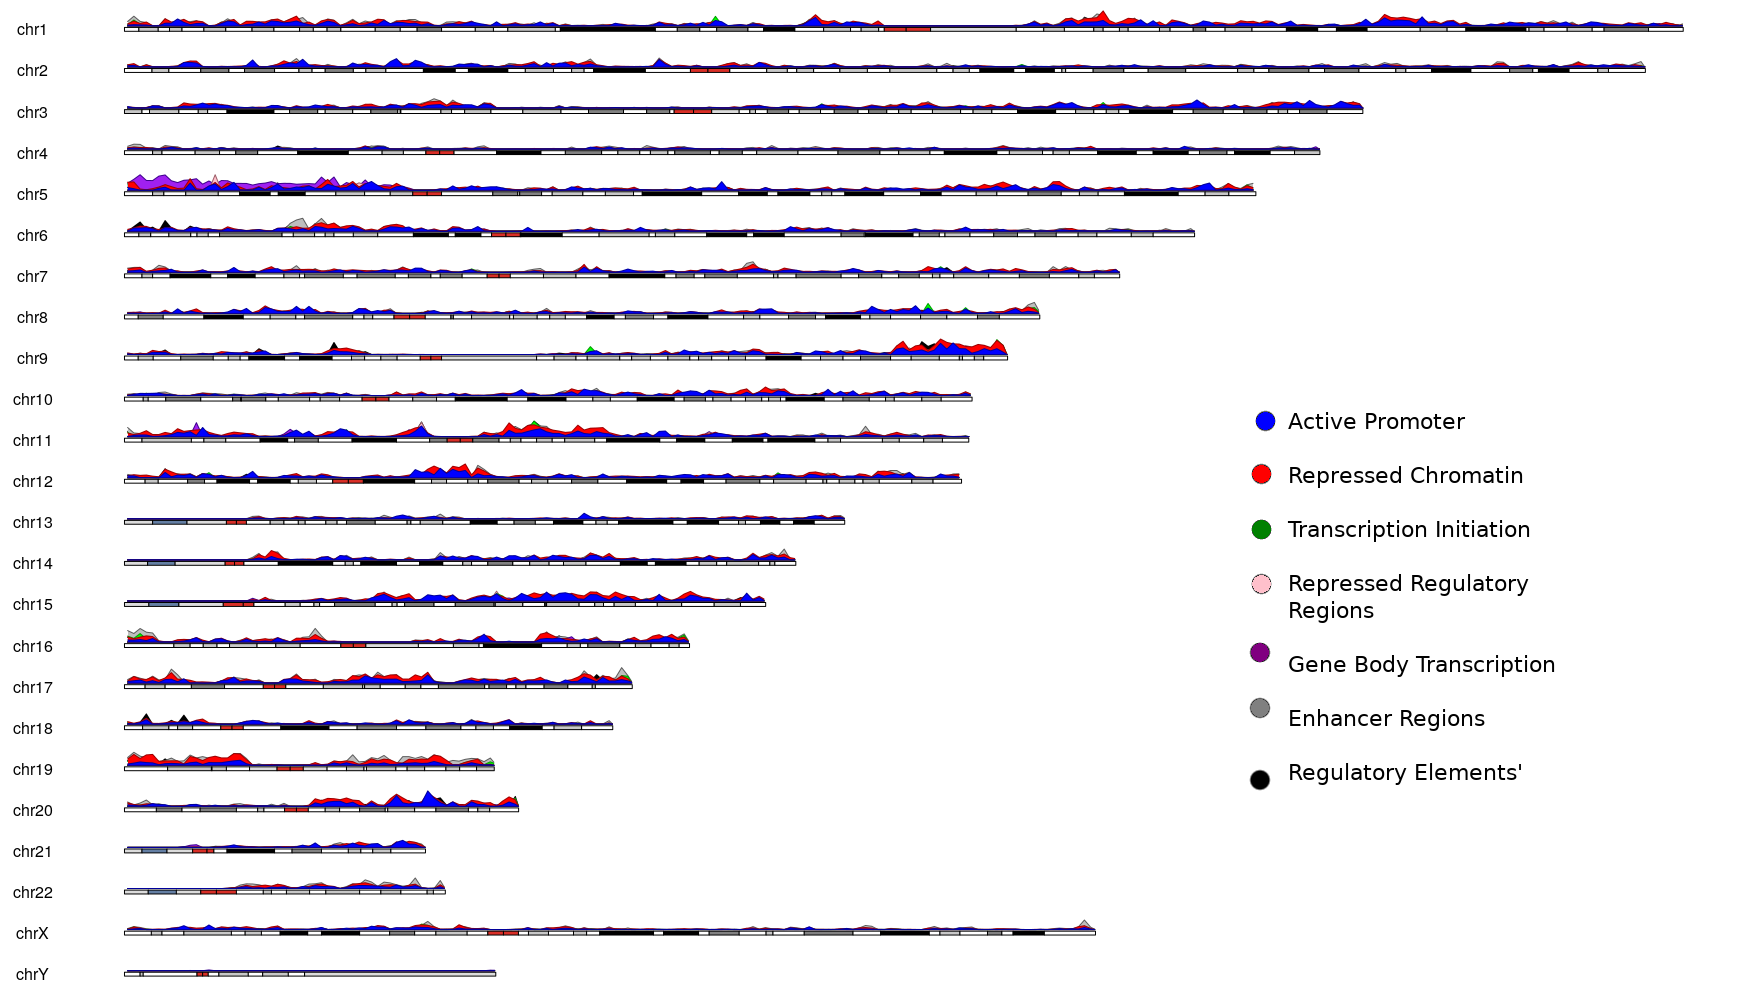
\includegraphics[width=\textwidth]{Figures/cover/signatures_density.png}
    \caption[Signatures density along the chromosomes]{\textbf{Signatures density along the chromosomes}. Figure description. Lots of things. Lots of things. Lots of things. Lots of things.Lots of things. Lots of things. Lots of things. Lots of things.Lots of things. Lots of things. Lots of things. Lots of things.}
    \label{fig:W_density}
\end{sidewaysfigure}

\medskip

Taking chromosome 4 as an example, we can better see the distribution of the signatures in Figure~\ref{fig:chr4}. In this case, Hela-S3 results are presented and we can observe a few patterns:

\begin{itemize}
    \item All the signatures but 5 (Gene Body Transcription) follow a similar distribution along the chromosome 4.
    \item Signatures 1 (Active Promoter), 3 (Transcription Initiation), 4 (Repressed Regulatory Regions) and 6 (Enhancer regions) share a even similar profile. Being these signatures related to the gene activation, the observation for chromosome 4 go along with the involved biological processes.
    \item In points where the signatures described in the last point are the lowest, signature 2 (Repressed Chromatin) presents peaks.
    \item Signature 5 (Gene Body Transcription) ilustrates a generaly low occurrence of bins assigned to the group in chromosome 4. Moreover, we see remarkable maximum peaks in the beginning and the end of the chromosome as well as the centromere.
    \item For signature 7 (Regulatory Elements), it looks like it is more dominant in the left arm of the chromosome 4.
\end{itemize}

% Chapter Template

\chapter{Discussion} % Main chapter title

\label{Discussion} % Change X to a consecutive number; for referencing this chapter elsewhere, use \ref{ChapterX}

%----------------------------------------------------------------------------------------
%	SECTION 1
%----------------------------------------------------------------------------------------

\section{Main Section 1}

Lorem ipsum dolor sit amet, consectetur adipiscing elit. Aliquam ultricies lacinia euismod. Nam tempus risus in dolor rhoncus in interdum enim tincidunt. Donec vel nunc neque. In condimentum ullamcorper quam non consequat. Fusce sagittis tempor feugiat. Fusce magna erat, molestie eu convallis ut, tempus sed arcu. Quisque molestie, ante a tincidunt ullamcorper, sapien enim dignissim lacus, in semper nibh erat lobortis purus. Integer dapibus ligula ac risus convallis pellentesque.

%-----------------------------------
%	SUBSECTION 1
%-----------------------------------
\subsection{Subsection 1}

Nunc posuere quam at lectus tristique eu ultrices augue venenatis. Vestibulum ante ipsum primis in faucibus orci luctus et ultrices posuere cubilia Curae; Aliquam erat volutpat. Vivamus sodales tortor eget quam adipiscing in vulputate ante ullamcorper. Sed eros ante, lacinia et sollicitudin et, aliquam sit amet augue. In hac habitasse platea dictumst.

%-----------------------------------
%	SUBSECTION 2
%-----------------------------------

\subsection{Subsection 2}
Morbi rutrum odio eget arcu adipiscing sodales. Aenean et purus a est pulvinar pellentesque. Cras in elit neque, quis varius elit. Phasellus fringilla, nibh eu tempus venenatis, dolor elit posuere quam, quis adipiscing urna leo nec orci. Sed nec nulla auctor odio aliquet consequat. Ut nec nulla in ante ullamcorper aliquam at sed dolor. Phasellus fermentum magna in augue gravida cursus. Cras sed pretium lorem. Pellentesque eget ornare odio. Proin accumsan, massa viverra cursus pharetra, ipsum nisi lobortis velit, a malesuada dolor lorem eu neque.

%----------------------------------------------------------------------------------------
%	SECTION 2
%----------------------------------------------------------------------------------------

\section{Main Section 2}

Sed ullamcorper quam eu nisl interdum at interdum enim egestas. Aliquam placerat justo sed lectus lobortis ut porta nisl porttitor. Vestibulum mi dolor, lacinia molestie gravida at, tempus vitae ligula. Donec eget quam sapien, in viverra eros. Donec pellentesque justo a massa fringilla non vestibulum metus vestibulum. Vestibulum in orci quis felis tempor lacinia. Vivamus ornare ultrices facilisis. Ut hendrerit volutpat vulputate. Morbi condimentum venenatis augue, id porta ipsum vulputate in. Curabitur luctus tempus justo. Vestibulum risus lectus, adipiscing nec condimentum quis, condimentum nec nisl. Aliquam dictum sagittis velit sed iaculis. Morbi tristique augue sit amet nulla pulvinar id facilisis ligula mollis. Nam elit libero, tincidunt ut aliquam at, molestie in quam. Aenean rhoncus vehicula hendrerit.

% % Chapter 1

\chapter{Chapter 1} % Main chapter title

\label{Chapter1} % For referencing the chapter elsewhere, use \ref{Introduction}

%----------------------------------------------------------------------------------------

% Define some commands to keep the formatting separated from the content
\newcommand{\keyword}[1]{\textbf{#1}}
\newcommand{\tabhead}[1]{\textbf{#1}}
\newcommand{\code}[1]{\texttt{#1}}
\newcommand{\file}[1]{\texttt{\bfseries#1}}
\newcommand{\option}[1]{\texttt{\itshape#1}}

%----------------------------------------------------------------------------------------

\section{Epigenetics}
Welcome to this \LaTeX{} Thesis Template, a beautiful and easy to use template for writing a thesis using the \LaTeX{} typesetting system.

If you are writing a thesis (or will be in the future) and its subject is technical or mathematical (though it doesn't have to be), then creating it in \LaTeX{} is highly recommended as a way to make sure you can just get down to the essential writing without having to worry over formatting or wasting time arguing with your word processor.

\LaTeX{} is easily able to professionally typeset documents that run to hundreds or thousands of pages long. With simple mark-up commands, it automatically sets out the table of contents, margins, page headers and footers and keeps the formatting consistent and beautiful. One of its main strengths is the way it can easily typeset mathematics, even \emph{heavy} mathematics. Even if those equations are the most horribly twisted and most difficult mathematical problems that can only be solved on a super-computer, you can at least count on \LaTeX{} to make them look stunning.

%----------------------------------------------------------------------------------------

\section{Non-negative Matrix Factorization}

\LaTeX{} is not a \textsc{wysiwyg} (What You See is What You Get) program, unlike word processors such as Microsoft Word or Apple's Pages. Instead, a document written for \LaTeX{} is actually a simple, plain text file that contains \emph{no formatting}. You tell \LaTeX{} how you want the formatting in the finished document by writing in simple commands amongst the text, for example, if I want to use \emph{italic text for emphasis}, I write the \verb|\emph{text}| command and put the text I want in italics in between the curly braces. This means that \LaTeX{} is a \enquote{mark-up} language, very much like HTML.

\subsection{A (not so short) Introduction to \LaTeX{}}

If you are new to \LaTeX{}, there is a very good eBook -- freely available online as a PDF file -- called, \enquote{The Not So Short Introduction to \LaTeX{}}. The book's title is typically shortened to just \emph{lshort}. You can download the latest version (as it is occasionally updated) from here:
\url{http://www.ctan.org/tex-archive/info/lshort/english/lshort.pdf}

It is also available in several other languages. Find yours from the list on this page: \url{http://www.ctan.org/tex-archive/info/lshort/}

It is recommended to take a little time out to learn how to use \LaTeX{} by creating several, small `test' documents, or having a close look at several templates on:\\
\url{http://www.LaTeXTemplates.com}\\
Making the effort now means you're not stuck learning the system when what you \emph{really} need to be doing is writing your thesis.

\subsection{A Short Math Guide for \LaTeX{}}

If you are writing a technical or mathematical thesis, then you may want to read the document by the AMS (American Mathematical Society) called, \enquote{A Short Math Guide for \LaTeX{}}. It can be found online here:
\url{http://www.ams.org/tex/amslatex.html}
under the \enquote{Additional Documentation} section towards the bottom of the page.

\subsection{Common \LaTeX{} Math Symbols}
There are a multitude of mathematical symbols available for \LaTeX{} and it would take a great effort to learn the commands for them all. The most common ones you are likely to use are shown on this page:
\url{http://www.sunilpatel.co.uk/latex-type/latex-math-symbols/}

You can use this page as a reference or crib sheet, the symbols are rendered as large, high quality images so you can quickly find the \LaTeX{} command for the symbol you need.

\subsection{\LaTeX{} on a Mac}

The \LaTeX{} distribution is available for many systems including Windows, Linux and Mac OS X. The package for OS X is called MacTeX and it contains all the applications you need -- bundled together and pre-customized -- for a fully working \LaTeX{} environment and work flow.

MacTeX includes a custom dedicated \LaTeX{} editor called TeXShop for writing your `\file{.tex}' files and BibDesk: a program to manage your references and create your bibliography section just as easily as managing songs and creating playlists in iTunes.

%----------------------------------------------------------------------------------------

\section{Getting Started with this Template}

If you are familiar with \LaTeX{}, then you should explore the directory structure of the template and then proceed to place your own information into the \emph{THESIS INFORMATION} block of the \file{main.tex} file. You can then modify the rest of this file to your unique specifications based on your degree/university. Section \ref{FillingFile} on page \pageref{FillingFile} will help you do this. Make sure you also read section \ref{ThesisConventions} about thesis conventions to get the most out of this template.

If you are new to \LaTeX{} it is recommended that you carry on reading through the rest of the information in this document.

Before you begin using this template you should ensure that its style complies with the thesis style guidelines imposed by your institution. In most cases this template style and layout will be suitable. If it is not, it may only require a small change to bring the template in line with your institution's recommendations. These modifications will need to be done on the \file{MastersDoctoralThesis.cls} file.

\subsection{About this Template}

This \LaTeX{} Thesis Template is originally based and created around a \LaTeX{} style file created by Steve R.\ Gunn from the University of Southampton (UK), department of Electronics and Computer Science. You can find his original thesis style file at his site, here:
\url{http://www.ecs.soton.ac.uk/~srg/softwaretools/document/templates/}

Steve's \file{ecsthesis.cls} was then taken by Sunil Patel who modified it by creating a skeleton framework and folder structure to place the thesis files in. The resulting template can be found on Sunil's site here:
\url{http://www.sunilpatel.co.uk/thesis-template}

Sunil's template was made available through \url{http://www.LaTeXTemplates.com} where it was modified many times based on user requests and questions. Version 2.0 and onwards of this template represents a major modification to Sunil's template and is, in fact, hardly recognisable. The work to make version 2.0 possible was carried out by \href{mailto:vel@latextemplates.com}{Vel} and Johannes Böttcher.

%----------------------------------------------------------------------------------------

\section{What this Template Includes}

\subsection{Folders}

This template comes as a single zip file that expands out to several files and folders. The folder names are mostly self-explanatory:

\keyword{Appendices} -- this is the folder where you put the appendices. Each appendix should go into its own separate \file{.tex} file. An example and template are included in the directory.

\keyword{Chapters} -- this is the folder where you put the thesis chapters. A thesis usually has about six chapters, though there is no hard rule on this. Each chapter should go in its own separate \file{.tex} file and they can be split as:
\begin{itemize}
\item Chapter 1: Introduction to the thesis topic
\item Chapter 2: Background information and theory
\item Chapter 3: (Laboratory) experimental setup
\item Chapter 4: Details of experiment 1
\item Chapter 5: Details of experiment 2
\item Chapter 6: Discussion of the experimental results
\item Chapter 7: Conclusion and future directions
\end{itemize}
This chapter layout is specialised for the experimental sciences, your discipline may be different.

\keyword{Figures} -- this folder contains all figures for the thesis. These are the final images that will go into the thesis document.

\subsection{Files}

Included are also several files, most of them are plain text and you can see their contents in a text editor. After initial compilation, you will see that more auxiliary files are created by \LaTeX{} or BibTeX and which you don't need to delete or worry about:

\keyword{example.bib} -- this is an important file that contains all the bibliographic information and references that you will be citing in the thesis for use with BibTeX. You can write it manually, but there are reference manager programs available that will create and manage it for you. Bibliographies in \LaTeX{} are a large subject and you may need to read about BibTeX before starting with this. Many modern reference managers will allow you to export your references in BibTeX format which greatly eases the amount of work you have to do.

\keyword{MastersDoctoralThesis.cls} -- this is an important file. It is the class file that tells \LaTeX{} how to format the thesis.

\keyword{main.pdf} -- this is your beautifully typeset thesis (in the PDF file format) created by \LaTeX{}. It is supplied in the PDF with the template and after you compile the template you should get an identical version.

\keyword{main.tex} -- this is an important file. This is the file that you tell \LaTeX{} to compile to produce your thesis as a PDF file. It contains the framework and constructs that tell \LaTeX{} how to layout the thesis. It is heavily commented so you can read exactly what each line of code does and why it is there. After you put your own information into the \emph{THESIS INFORMATION} block -- you have now started your thesis!

Files that are \emph{not} included, but are created by \LaTeX{} as auxiliary files include:

\keyword{main.aux} -- this is an auxiliary file generated by \LaTeX{}, if it is deleted \LaTeX{} simply regenerates it when you run the main \file{.tex} file.

\keyword{main.bbl} -- this is an auxiliary file generated by BibTeX, if it is deleted, BibTeX simply regenerates it when you run the \file{main.aux} file. Whereas the \file{.bib} file contains all the references you have, this \file{.bbl} file contains the references you have actually cited in the thesis and is used to build the bibliography section of the thesis.

\keyword{main.blg} -- this is an auxiliary file generated by BibTeX, if it is deleted BibTeX simply regenerates it when you run the main \file{.aux} file.

\keyword{main.lof} -- this is an auxiliary file generated by \LaTeX{}, if it is deleted \LaTeX{} simply regenerates it when you run the main \file{.tex} file. It tells \LaTeX{} how to build the \emph{List of Figures} section.

\keyword{main.log} -- this is an auxiliary file generated by \LaTeX{}, if it is deleted \LaTeX{} simply regenerates it when you run the main \file{.tex} file. It contains messages from \LaTeX{}, if you receive errors and warnings from \LaTeX{}, they will be in this \file{.log} file.

\keyword{main.lot} -- this is an auxiliary file generated by \LaTeX{}, if it is deleted \LaTeX{} simply regenerates it when you run the main \file{.tex} file. It tells \LaTeX{} how to build the \emph{List of Tables} section.

\keyword{main.out} -- this is an auxiliary file generated by \LaTeX{}, if it is deleted \LaTeX{} simply regenerates it when you run the main \file{.tex} file.

So from this long list, only the files with the \file{.bib}, \file{.cls} and \file{.tex} extensions are the most important ones. The other auxiliary files can be ignored or deleted as \LaTeX{} and BibTeX will regenerate them.

%----------------------------------------------------------------------------------------

\section{Filling in Your Information in the \file{main.tex} File}\label{FillingFile}

You will need to personalise the thesis template and make it your own by filling in your own information. This is done by editing the \file{main.tex} file in a text editor or your favourite LaTeX environment.

Open the file and scroll down to the third large block titled \emph{THESIS INFORMATION} where you can see the entries for \emph{University Name}, \emph{Department Name}, etc \ldots

Fill out the information about yourself, your group and institution. You can also insert web links, if you do, make sure you use the full URL, including the \code{http://} for this. If you don't want these to be linked, simply remove the \verb|\href{url}{name}| and only leave the name.

When you have done this, save the file and recompile \code{main.tex}. All the information you filled in should now be in the PDF, complete with web links. You can now begin your thesis proper!

%----------------------------------------------------------------------------------------

\section{The \code{main.tex} File Explained}

The \file{main.tex} file contains the structure of the thesis. There are plenty of written comments that explain what pages, sections and formatting the \LaTeX{} code is creating. Each major document element is divided into commented blocks with titles in all capitals to make it obvious what the following bit of code is doing. Initially there seems to be a lot of \LaTeX{} code, but this is all formatting, and it has all been taken care of so you don't have to do it.

Begin by checking that your information on the title page is correct. For the thesis declaration, your institution may insist on something different than the text given. If this is the case, just replace what you see with what is required in the \emph{DECLARATION PAGE} block.

Then comes a page which contains a funny quote. You can put your own, or quote your favourite scientist, author, person, and so on. Make sure to put the name of the person who you took the quote from.

Following this is the abstract page which summarises your work in a condensed way and can almost be used as a standalone document to describe what you have done. The text you write will cause the heading to move up so don't worry about running out of space.

Next come the acknowledgements. On this page, write about all the people who you wish to thank (not forgetting parents, partners and your advisor/supervisor).

The contents pages, list of figures and tables are all taken care of for you and do not need to be manually created or edited. The next set of pages are more likely to be optional and can be deleted since they are for a more technical thesis: insert a list of abbreviations you have used in the thesis, then a list of the physical constants and numbers you refer to and finally, a list of mathematical symbols used in any formulae. Making the effort to fill these tables means the reader has a one-stop place to refer to instead of searching the internet and references to try and find out what you meant by certain abbreviations or symbols.

The list of symbols is split into the Roman and Greek alphabets. Whereas the abbreviations and symbols ought to be listed in alphabetical order (and this is \emph{not} done automatically for you) the list of physical constants should be grouped into similar themes.

The next page contains a one line dedication. Who will you dedicate your thesis to?

Finally, there is the block where the chapters are included. Uncomment the lines (delete the \code{\%} character) as you write the chapters. Each chapter should be written in its own file and put into the \emph{Chapters} folder and named \file{Chapter1}, \file{Chapter2}, etc\ldots Similarly for the appendices, uncomment the lines as you need them. Each appendix should go into its own file and placed in the \emph{Appendices} folder.

After the preamble, chapters and appendices finally comes the bibliography. The bibliography style (called \option{authoryear}) is used for the bibliography and is a fully featured style that will even include links to where the referenced paper can be found online. Do not underestimate how grateful your reader will be to find that a reference to a paper is just a click away. Of course, this relies on you putting the URL information into the BibTeX file in the first place.

%----------------------------------------------------------------------------------------

\section{Thesis Features and Conventions}\label{ThesisConventions}

To get the best out of this template, there are a few conventions that you may want to follow.

One of the most important (and most difficult) things to keep track of in such a long document as a thesis is consistency. Using certain conventions and ways of doing things (such as using a Todo list) makes the job easier. Of course, all of these are optional and you can adopt your own method.

\subsection{Printing Format}

This thesis template is designed for double sided printing (i.e. content on the front and back of pages) as most theses are printed and bound this way. Switching to one sided printing is as simple as uncommenting the \option{oneside} option of the \code{documentclass} command at the top of the \file{main.tex} file. You may then wish to adjust the margins to suit specifications from your institution.

The headers for the pages contain the page number on the outer side (so it is easy to flick through to the page you want) and the chapter name on the inner side.

The text is set to 11 point by default with single line spacing, again, you can tune the text size and spacing should you want or need to using the options at the very start of \file{main.tex}. The spacing can be changed similarly by replacing the \option{singlespacing} with \option{onehalfspacing} or \option{doublespacing}.

\subsection{Using US Letter Paper}

The paper size used in the template is A4, which is the standard size in Europe. If you are using this thesis template elsewhere and particularly in the United States, then you may have to change the A4 paper size to the US Letter size. This can be done in the margins settings section in \file{main.tex}.

Due to the differences in the paper size, the resulting margins may be different to what you like or require (as it is common for institutions to dictate certain margin sizes). If this is the case, then the margin sizes can be tweaked by modifying the values in the same block as where you set the paper size. Now your document should be set up for US Letter paper size with suitable margins.

\subsection{References}

The \code{biblatex} package is used to format the bibliography and inserts references such as this one \parencite{Reference1}. The options used in the \file{main.tex} file mean that the in-text citations of references are formatted with the author(s) listed with the date of the publication. Multiple references are separated by semicolons (e.g. \parencite{Reference2, Reference1}) and references with more than three authors only show the first author with \emph{et al.} indicating there are more authors (e.g. \parencite{Reference3}). This is done automatically for you. To see how you use references, have a look at the \file{Chapter1.tex} source file. Many reference managers allow you to simply drag the reference into the document as you type.

Scientific references should come \emph{before} the punctuation mark if there is one (such as a comma or period). The same goes for footnotes\footnote{Such as this footnote, here down at the bottom of the page.}. You can change this but the most important thing is to keep the convention consistent throughout the thesis. Footnotes themselves should be full, descriptive sentences (beginning with a capital letter and ending with a full stop). The APA6 states: \enquote{Footnote numbers should be superscripted, [...], following any punctuation mark except a dash.} The Chicago manual of style states: \enquote{A note number should be placed at the end of a sentence or clause. The number follows any punctuation mark except the dash, which it precedes. It follows a closing parenthesis.}

The bibliography is typeset with references listed in alphabetical order by the first author's last name. This is similar to the APA referencing style. To see how \LaTeX{} typesets the bibliography, have a look at the very end of this document (or just click on the reference number links in in-text citations).

\subsubsection{A Note on bibtex}

The bibtex backend used in the template by default does not correctly handle unicode character encoding (i.e. "international" characters). You may see a warning about this in the compilation log and, if your references contain unicode characters, they may not show up correctly or at all. The solution to this is to use the biber backend instead of the outdated bibtex backend. This is done by finding this in \file{main.tex}: \option{backend=bibtex} and changing it to \option{backend=biber}. You will then need to delete all auxiliary BibTeX files and navigate to the template directory in your terminal (command prompt). Once there, simply type \code{biber main} and biber will compile your bibliography. You can then compile \file{main.tex} as normal and your bibliography will be updated. An alternative is to set up your LaTeX editor to compile with biber instead of bibtex, see \href{http://tex.stackexchange.com/questions/154751/biblatex-with-biber-configuring-my-editor-to-avoid-undefined-citations/}{here} for how to do this for various editors.

\subsection{Tables}

Tables are an important way of displaying your results, below is an example table which was generated with this code:

{\small
\begin{verbatim}
\begin{table}
\caption{The effects of treatments X and Y on the four groups studied.}
\label{tab:treatments}
\centering
\begin{tabular}{l l l}
\toprule
\tabhead{Groups} & \tabhead{Treatment X} & \tabhead{Treatment Y} \\
\midrule
1 & 0.2 & 0.8\\
2 & 0.17 & 0.7\\
3 & 0.24 & 0.75\\
4 & 0.68 & 0.3\\
\bottomrule\\
\end{tabular}
\end{table}
\end{verbatim}
}

\begin{table}
\caption{The effects of treatments X and Y on the four groups studied.}
\label{tab:treatments}
\centering
\begin{tabular}{l l l}
\toprule
\tabhead{Groups} & \tabhead{Treatment X} & \tabhead{Treatment Y} \\
\midrule
1 & 0.2 & 0.8\\
2 & 0.17 & 0.7\\
3 & 0.24 & 0.75\\
4 & 0.68 & 0.3\\
\bottomrule\\
\end{tabular}
\end{table}

You can reference tables with \verb|\ref{<label>}| where the label is defined within the table environment. See \file{Chapter1.tex} for an example of the label and citation (e.g. Table~\ref{tab:treatments}).

\subsection{Figures}

There will hopefully be many figures in your thesis (that should be placed in the \emph{Figures} folder). The way to insert figures into your thesis is to use a code template like this:
\begin{verbatim}
\begin{figure}
\centering

\includegraphics{Figures/Electron}
\decoRule
\caption[An Electron]{An electron (artist's impression).}
\label{fig:Electron}
\end{figure}
\end{verbatim}
Also look in the source file. Putting this code into the source file produces the picture of the electron that you can see in the figure below.

\begin{figure}[th]
\centering

\includegraphics{Figures/Electron}
\decoRule
\caption[An Electron]{An electron (artist's impression).}
\label{fig:Electron}
\end{figure}

Sometimes figures don't always appear where you write them in the source. The placement depends on how much space there is on the page for the figure. Sometimes there is not enough room to fit a figure directly where it should go (in relation to the text) and so \LaTeX{} puts it at the top of the next page. Positioning figures is the job of \LaTeX{} and so you should only worry about making them look good!

Figures usually should have captions just in case you need to refer to them (such as in Figure~\ref{fig:Electron}). The \verb|\caption| command contains two parts, the first part, inside the square brackets is the title that will appear in the \emph{List of Figures}, and so should be short. The second part in the curly brackets should contain the longer and more descriptive caption text.

The \verb|\decoRule| command is optional and simply puts an aesthetic horizontal line below the image. If you do this for one image, do it for all of them.

\LaTeX{} is capable of using images in pdf, jpg and png format.

\subsection{Typesetting mathematics}

If your thesis is going to contain heavy mathematical content, be sure that \LaTeX{} will make it look beautiful, even though it won't be able to solve the equations for you.

The \enquote{Not So Short Introduction to \LaTeX} (available on \href{http://www.ctan.org/tex-archive/info/lshort/english/lshort.pdf}{CTAN}) should tell you everything you need to know for most cases of typesetting mathematics. If you need more information, a much more thorough mathematical guide is available from the AMS called, \enquote{A Short Math Guide to \LaTeX} and can be downloaded from:
\url{ftp://ftp.ams.org/pub/tex/doc/amsmath/short-math-guide.pdf}

There are many different \LaTeX{} symbols to remember, luckily you can find the most common symbols in \href{http://ctan.org/pkg/comprehensive}{The Comprehensive \LaTeX~Symbol List}.

You can write an equation, which is automatically given an equation number by \LaTeX{} like this:
\begin{verbatim}
\begin{equation}
E = mc^{2}
\label{eqn:Einstein}
\end{equation}
\end{verbatim}

This will produce Einstein's famous energy-matter equivalence equation:
\begin{equation}
E = mc^{2}
\label{eqn:Einstein}
\end{equation}

All equations you write (which are not in the middle of paragraph text) are automatically given equation numbers by \LaTeX{}. If you don't want a particular equation numbered, use the unnumbered form:
\begin{verbatim}
\[ a^{2}=4 \]
\end{verbatim}

%----------------------------------------------------------------------------------------

\section{Sectioning and Subsectioning}

You should break your thesis up into nice, bite-sized sections and subsections. \LaTeX{} automatically builds a table of Contents by looking at all the \verb|\chapter{}|, \verb|\section{}|  and \verb|\subsection{}| commands you write in the source.

The Table of Contents should only list the sections to three (3) levels. A \verb|chapter{}| is level zero (0). A \verb|\section{}| is level one (1) and so a \verb|\subsection{}| is level two (2). In your thesis it is likely that you will even use a \verb|subsubsection{}|, which is level three (3). The depth to which the Table of Contents is formatted is set within \file{MastersDoctoralThesis.cls}. If you need this changed, you can do it in \file{main.tex}.

%----------------------------------------------------------------------------------------

\section{In Closing}

You have reached the end of this mini-guide. You can now rename or overwrite this pdf file and begin writing your own \file{Chapter1.tex} and the rest of your thesis. The easy work of setting up the structure and framework has been taken care of for you. It's now your job to fill it out!

Good luck and have lots of fun!

\begin{flushright}
Guide written by ---\\
Sunil Patel: \href{http://www.sunilpatel.co.uk}{www.sunilpatel.co.uk}\\
Vel: \href{http://www.LaTeXTemplates.com}{LaTeXTemplates.com}
\end{flushright}


%----------------------------------------------------------------------------------------
%	THESIS CONTENT - APPENDICES
%----------------------------------------------------------------------------------------

\appendix % Cue to tell LaTeX that the following "chapters" are Appendices

% Include the appendices of the thesis as separate files from the Appendices folder
% Uncomment the lines as you write the Appendices

% Appendix A

\chapter{Frequently Asked Questions} % Main appendix title

\label{AppendixA} % For referencing this appendix elsewhere, use \ref{AppendixA}

\section{How do I change the colors of links?}

The color of links can be changed to your liking using:

{\small\verb!\hypersetup{urlcolor=red}!}, or

{\small\verb!\hypersetup{citecolor=green}!}, or

{\small\verb!\hypersetup{allcolor=blue}!}.

\noindent If you want to completely hide the links, you can use:

{\small\verb!\hypersetup{allcolors=.}!}, or even better: 

{\small\verb!\hypersetup{hidelinks}!}.

\noindent If you want to have obvious links in the PDF but not the printed text, use:

{\small\verb!\hypersetup{colorlinks=false}!}.

%\include{Appendices/AppendixB}
%\include{Appendices/AppendixC}

%----------------------------------------------------------------------------------------
%	BIBLIOGRAPHY
%----------------------------------------------------------------------------------------

\bibliography{mscthesis}
\bibliographystyle{apalike}

% \addcontentsline{toc}{chapter}{Bibliography}

% \printbibliography[heading=bibintoc]

%----------------------------------------------------------------------------------------

\end{document}
